\documentclass[main.tex]{subfiles}
\begin{document}

\section{Plugins}

\subsection{Design of Plugins}

Plugin is the law in the DARC Protocol, and all programs and operations within DARC must adhere to the restrictions imposed by all plugins. For an individual plugin, it is required to follow the logic outlined in the pseudo code below:

\begin{verbatim}
if plugin.condition:
    return plugin.returnType
\end{verbatim}

For the DARC protocol, the main difference between before-operation plugins and after-operation plugins lies in their return types. For before-operation plugins, as they determine whether a certain operation should be executed directly, rejected outright, or entered into a sandbox, they have three distinct return types that serve as their final decisions:

\begin{enumerate}
    \item \texttt{NO}. When the condition of a before-operation plugin is triggered, the plugin's decision for that operation is \texttt{NO}. This decision indicates that the plugin believes the operation violates its rules, and therefore, it is rejected outright before entering the sandbox for execution.

    \item \texttt{SANDBOX\_NEEDED}.   When the condition of a before-operation plugin is triggered, the plugin's decision for that operation is \texttt{SANDBOX\_NEEDED}. This decision indicates that the plugin cannot determine whether the operation should be accepted or rejected. The plugin is aware that the operation needs to be evaluated in the sandbox by after-operation plugins, and thus, the decision is made to let the operation proceed to the sandbox for further evaluation.

    \item \texttt{YES\_AND\_SKIP\_SANDBOX}. When the condition of a before-operation plugin is triggered, the plugin's decision for that operation is \texttt{YES\_AND\_SKIP\_SANDBOX}. This decision indicates that the plugin has determined that the operation should be approved and does not require execution in the sandbox. Therefore, the operation can proceed directly without going through the sandbox.
\end{enumerate}



For after-operation plugins, since the program has been executed in the sandbox and voting can commence, these plugins can have three return types as their final decisions:

\begin{enumerate}
    \item \texttt{NO}. When the condition of an after-operation plugin is triggered, the plugin's decision for the operation is \texttt{NO}. This decision indicates that the plugin believes the operation violates its rules and should be rejected outright.

    \item \texttt{VOTING\_NEEDED}. When the condition of an after-operation plugin is triggered, the plugin's decision for the operation is {VOTING\_NEEDED}. This decision indicates that the plugin believes the operation requires a vote, and the operation needs to initialize a voting item based on the voting rule specified by this plugin.

    \item \texttt{YES}. When the condition of an after-operation plugin is triggered, the plugin's decision for the operation is \texttt{YES}. This decision indicates that the plugin believes, based on its rules, the operation should be allowed to proceed.
\end{enumerate}


Each plugin has a condition node array, where condition nodes are stored in sequence. The root node corresponds to the node at index 0, which is the first node. The condition node array follows the following principles:

\begin{enumerate}
    \item The type of each node can be a boolean operator or an expression;
    \item For boolean operators, the type must be set as one of AND, OR, or NOT;
    \item For AND and OR operators, at least two valid child node indices must be specified in the child node list;
    \item For the NOT operator, a unique child node index must be specified in the child node list;
    \item For expression nodes, valid condition expression parameters consistent with the expression must be set;
    \item For expression nodes, the length of their child node list must be 0, meaning no child nodes are allowed.
\end{enumerate}

Figure \ref{fig:condition-nodes} is an example illustrating how a condition expression binary tree is serialized into a condition node array.

\begin{figure}
\centering
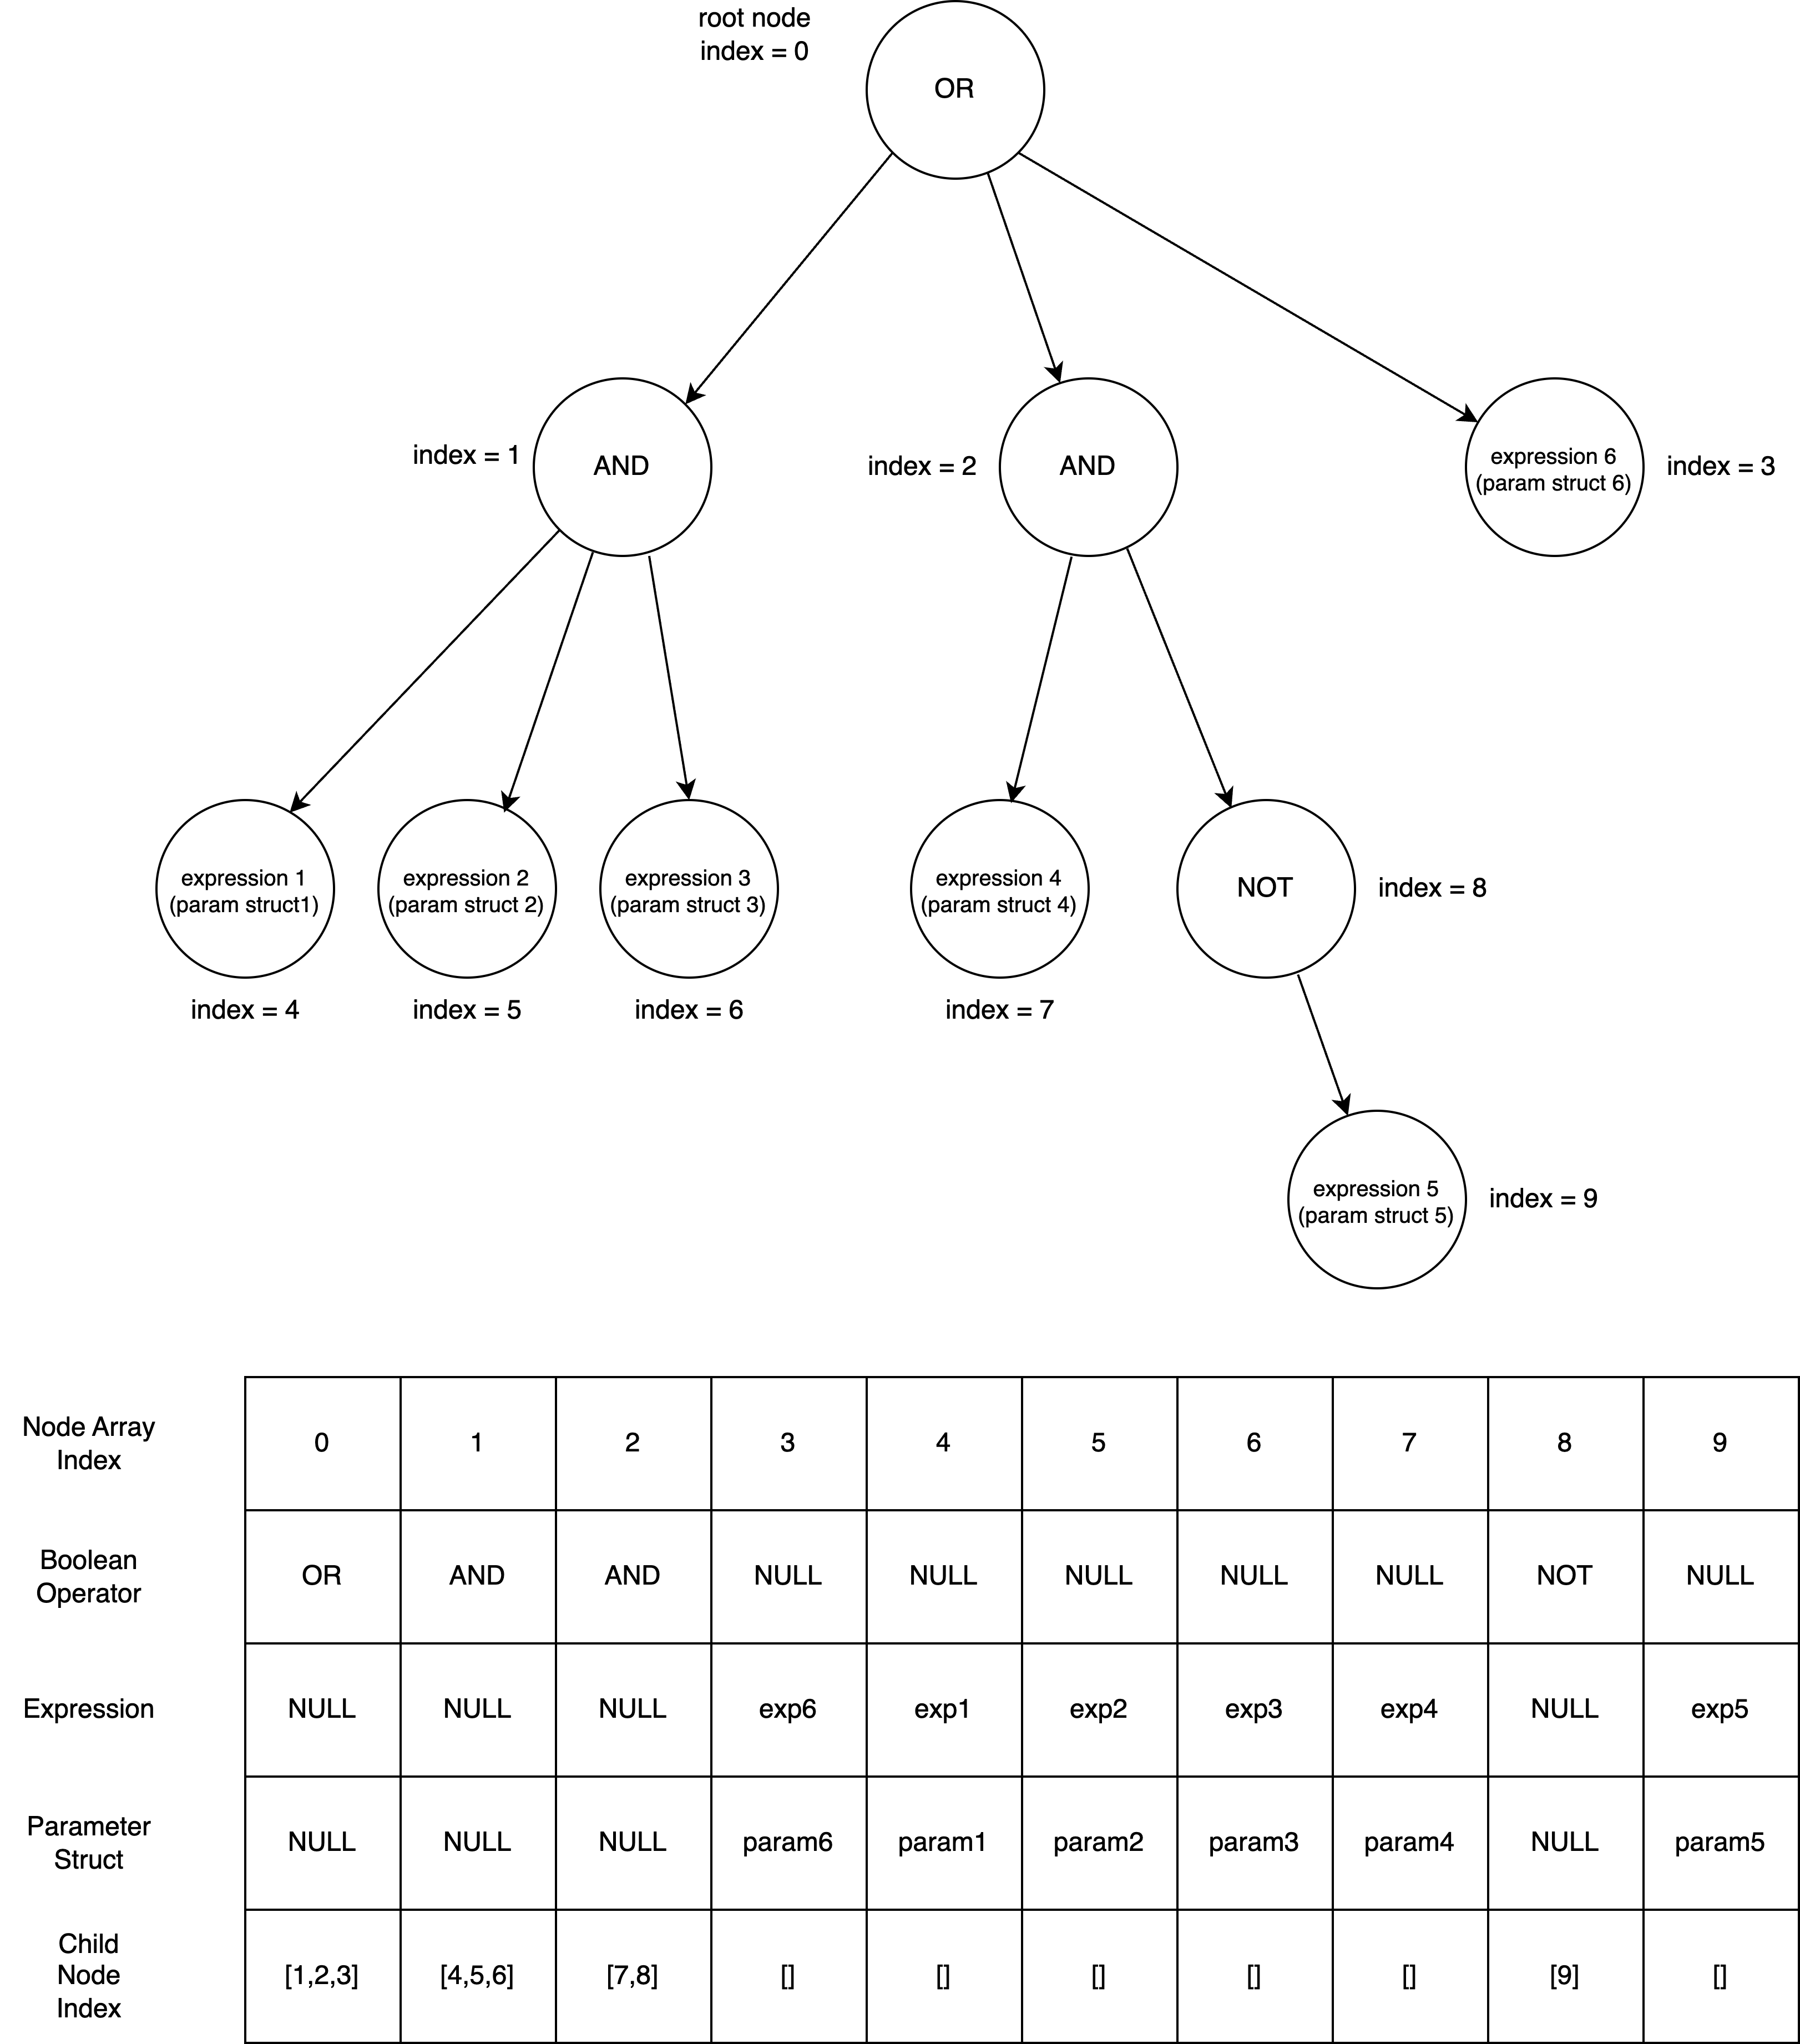
\includegraphics[width=1\linewidth]{plugin_condition_nodes.drawio.png}
\caption{\label{fig:condition-nodes}Condition Nodes and Expression Tree}
\end{figure}

Additionally, a plugin needs to set two parameters: one is the 'level', representing the priority of the plugin within the entire plugin system. For the same operation, the judgment system traverses all plugins, and it is possible that at least two or more plugins are triggered. In such cases, if the levels of the plugins are different, the judgment system will consider the plugin with the higher level as the final determination.

The other parameter is the 'voting rule index,' which points to a specific index in the voting rule array. When the final decision of a plugin is \texttt{VOTING\_NEEDED}, the plugin automatically requests the DARC protocol to use the voting rule indicated by the voting rule index for initializing the voting item. If the return type of the plugin is not \texttt{VOTING\_NEEDED}, the voting rule index will be ignored.



\subsection{The Plugin and the Judgement System}

For the DARC protocol, the judgment system needs to undergo two assessments: one through before-operation plugins and another after the program has run completely in the sandbox, followed by evaluation through after-operation plugins. The reason for this design is that, without a sandbox and relying solely on a set of plugins for judgment, it becomes challenging to anticipate the behavior of the program. As a result, it is not possible to protect against modifications to special states in the DARC protocol.

For example, in a DARC instance where shareholder X is required to permanently hold 15\% voting rights and 10\% dividend rights, when designing a plugin, it is impossible to predict the state of the DARC instance after the execution of operations like mint tokens or burn tokens. This uncertainty poses challenges in ensuring that shareholder X maintains permanent ownership of 15\% voting rights and 10\% dividend rights. Only by running the operation in the sandbox and then re-evaluating the state of the sandbox, can such modifications be prevented.

In another scenario, if there is a need to ensure that a DARC instance reserves 10,000 native tokens permanently before January 1, 2035, the correct detection and prevention of operations such as paying dividends or withdrawing cash can only be guaranteed by executing these operations in the sandbox. After all operations are completed in the sandbox, the judgment system performs a second evaluation through after-operation plugins. Without a sandbox and relying solely on plugins, the design of such a mechanism would be overly complex.


If there are only after-operation plugins and a sandbox without before-operation plugins, it would not be feasible. This is because the running cost of the sandbox is very high. It not only requires the program to run completely in the sandbox but also involves initializing the sandbox by fully replicating the internal state of the entire DARC instance. This process incurs a significant amount of gas fees.

For the majority of simple operations that can be approved without the need for running in the sandbox, it is more cost-effective to have rules established directly in before-operation plugins. These rules can leverage factors such as the operation, operator, timestamp, etc., for a straightforward approval or rejection, preventing them from entering the sandbox and saving costs.



For before-operation plugins, whenever a program is submitted to the DARC protocol, the judgment system sequentially checks each operation. For each operation, the judgment system traverses each before-operation plugin and obtains a single judgment result. Finally, it aggregates the results for all operations to determine the overall result for the entire program. This decision dictates whether the program needs to run in the sandbox (\texttt{SANDBOX\_NEEDED}), be rejected outright (\texttt{NO}), or run directly without the need for the sandbox (\texttt{YES\_AND\_SKIP\_SANDBOX}). For before-operation judgment, the following rules are followed:

\begin{enumerate}
    \item If any before-operation plugin returns a judgment result of \texttt{NO} for an operation, the entire program is rejected with a result of \texttt{NO}.
    \item If any before-operation plugin returns a judgment result of \texttt{SANDBOX\_NEEDED} for an operation, the entire program is required to run in the sandbox, and the result is \texttt{SANDBOX\_NEEDED}.
    \item If all before-operation plugins return a judgment result of \texttt{YES\_AND\_SKIP\_SANDBOX} for an operation, the entire program can skip the sandbox, and the result is \texttt{YES\_AND\_SKIP\_SANDBOX}.
\end{enumerate}


\begin{figure}
\centering
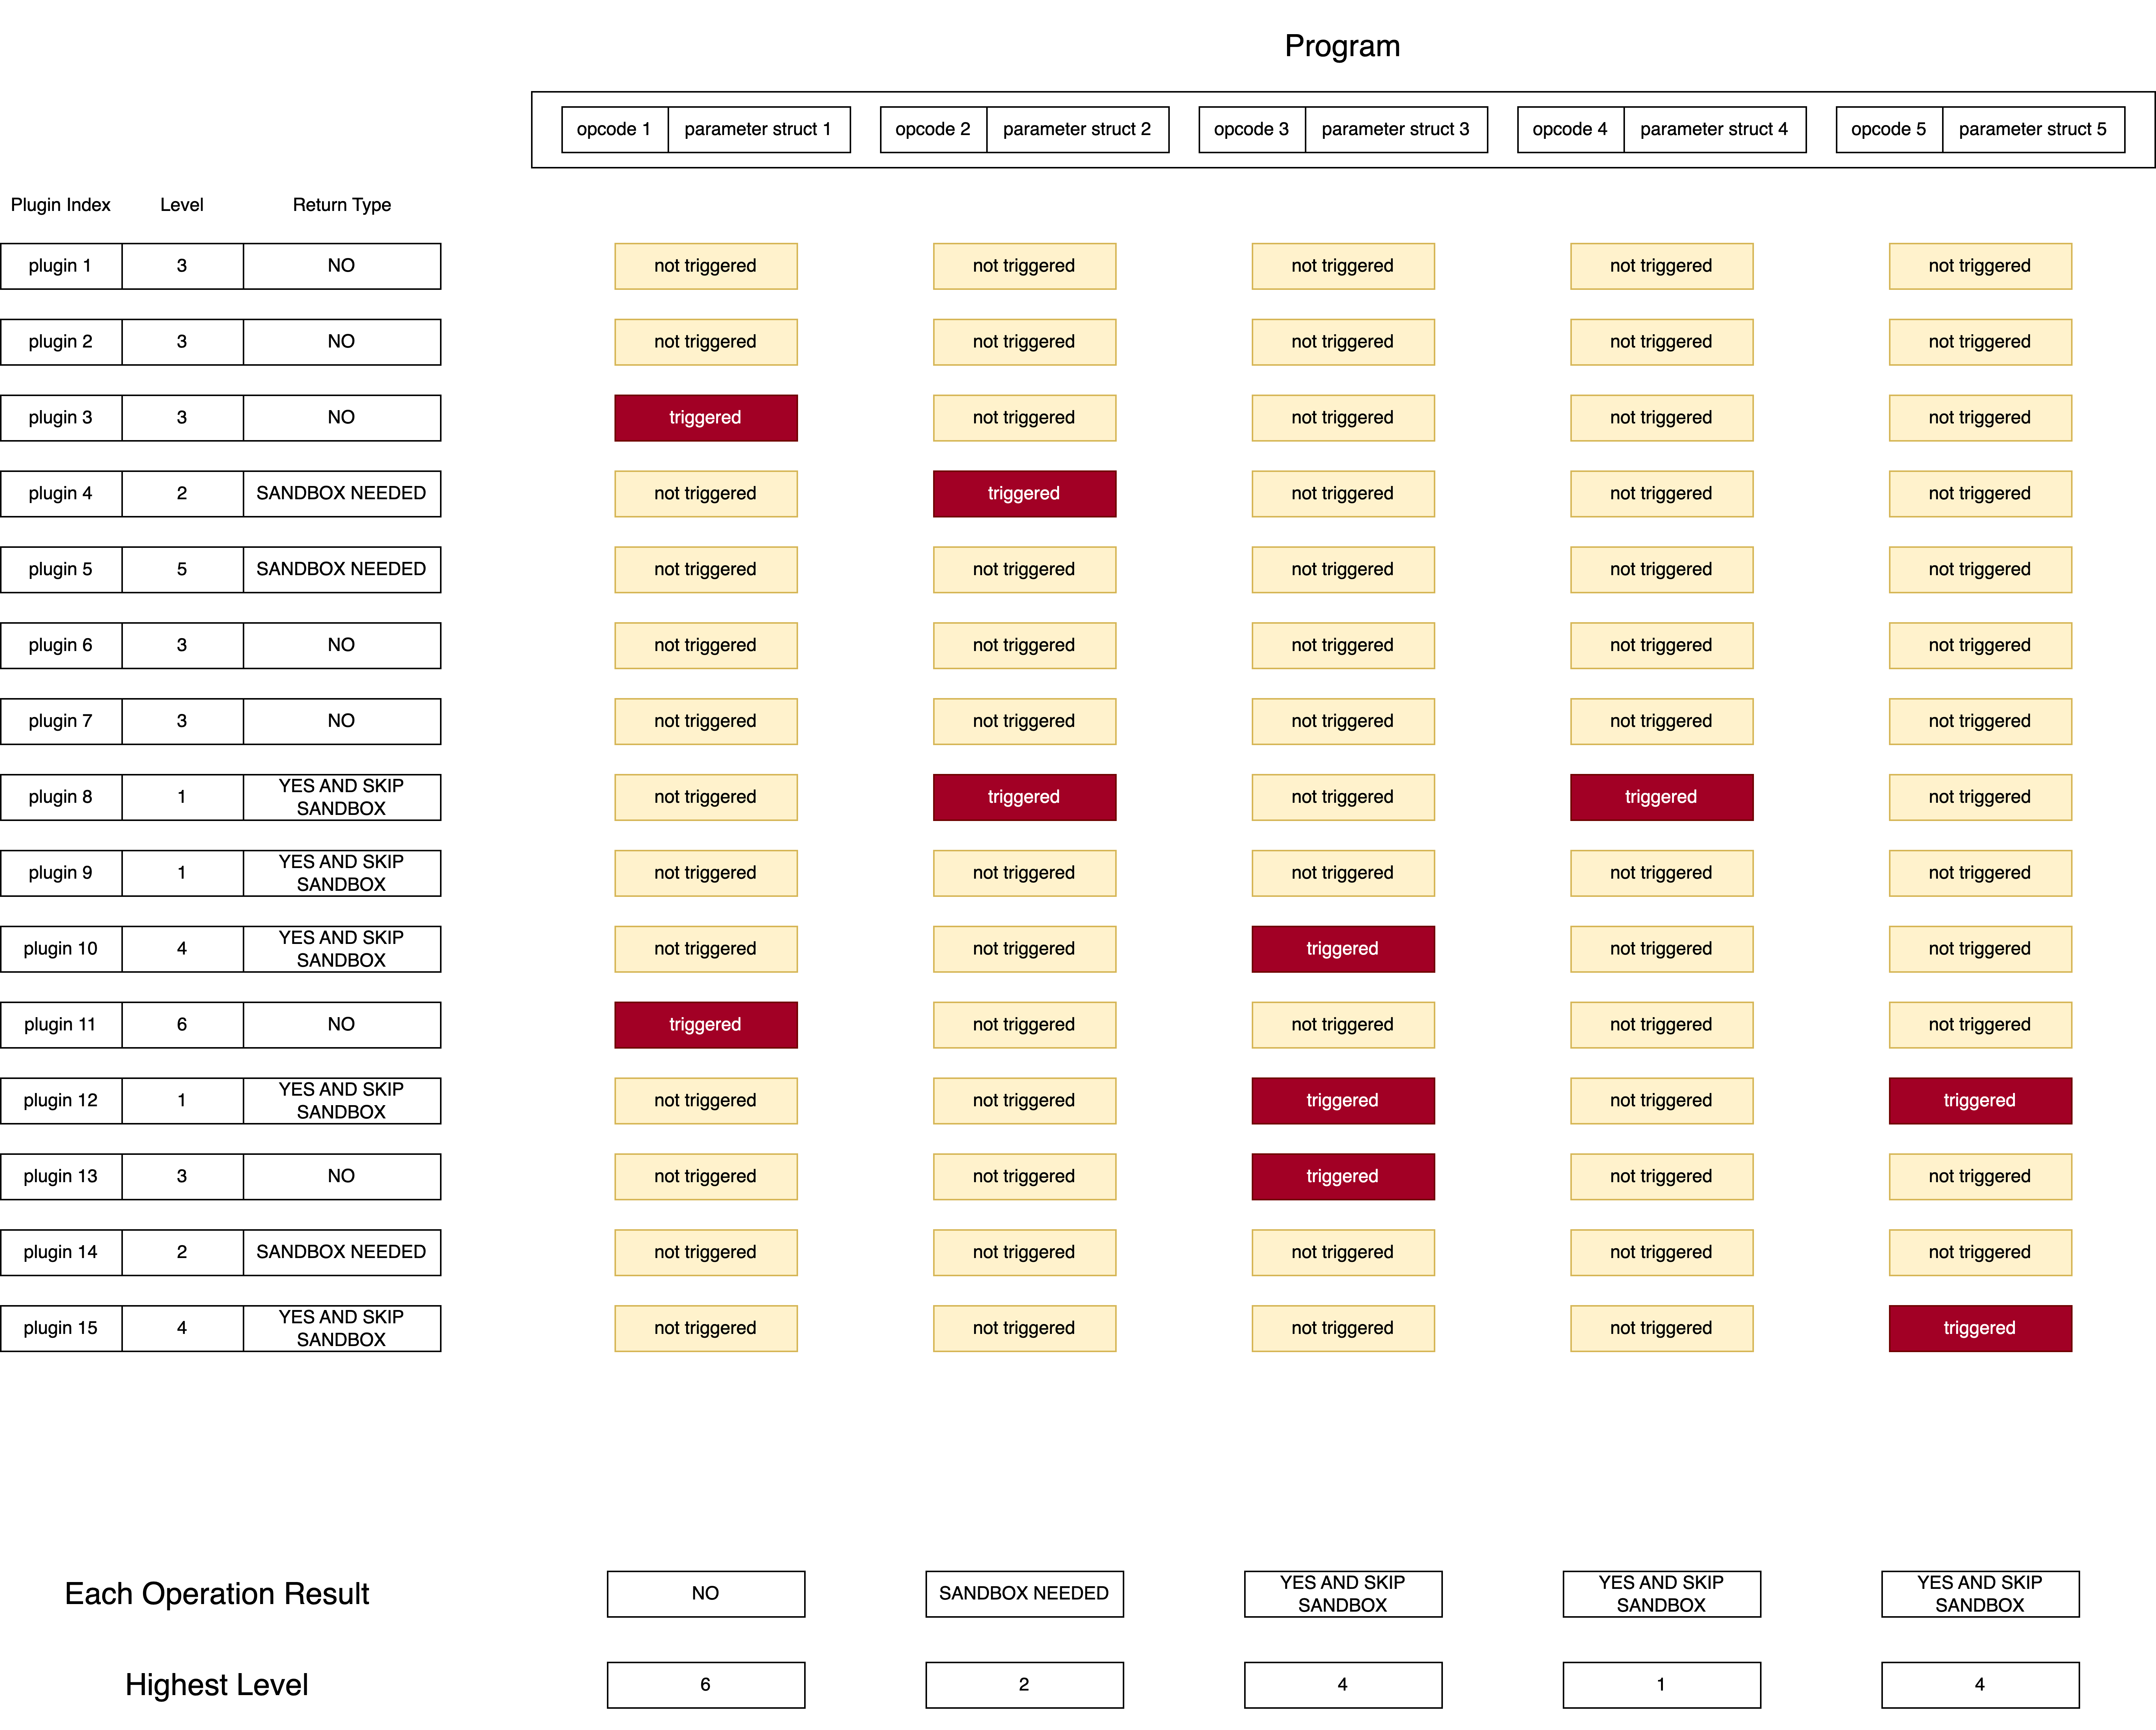
\includegraphics[width=1\linewidth]{judgement_plugin_levels_before_ops.drawio.png}
\caption{\label{fig:judgement-before-op}Judgement on program with before-operation plugins}
\end{figure}


Figure \ref{fig:judgement-before-op} illustrates how individual operations within a program are judged by before-operation plugins, resulting in judgment outcomes.











\subsection{Restriction Plugin System}

Restriction Plugin is the most important design in the DARC, since all the regulations are designed and implemented as plugins. Any operation can be aborted by the Decision Machine if it violates any of the restrictions or be denied by the voting system created by any restriction plugin. Each plugin is composed of two items: the condition and the return type. Before and after executing the operation by users, the Decision Virtual Machine will first go through the whole restriction plugin containers and check all the plugins sequentially. 



Algorithm 1 is the pseudo code of how the Decision Virtual Machine goes through the plugin system and makes the decisions.


\begin{algorithm}
\caption{Check if operation $P$ can be approved}
\begin{algorithmic} 


\FOR {$i = 0, 1, ..., \text{length}(S_{\text{plugin}}) $}
\IF {$ S_{\text{plugin}} [i].\text{condition} = \TRUE \And S_{\text{plugin}} [i].\text{return\textunderscore type} = \textbf{Absolutely\textunderscore Yes}  $}
\RETURN $ \TRUE $
\ELSIF{ $ S_{\text{plugin}} [i].\text{condition} = \TRUE \And S_{\text{plugin}} [i].\text{return\textunderscore type} = \textbf{No} $}
\RETURN $ \FALSE $
\ENDIF
\ENDFOR


\STATE {$\text{Voting\textunderscore Machine.initialize()}$}
\FOR {$i = 0, 1, ..., \text{length}(S_{\text{plugin}}) $}

\IF {$ S_{\text{plugin}} [i].\text{condition} = \TRUE \And S_{\text{plugin}} [i].\text{return\textunderscore type} = \textbf{Voting\textunderscore Needed} $}
\STATE ${\text{Voting\textunderscore Machine.add\textunderscore vote(}} S_{\text{plugin}} [i].\text{voting\textunderscore rule} \text{)} $
\ENDIF
\ENDFOR

\STATE $\text{Voting\textunderscore Machine.vote()} $

\RETURN $ \text{Voting\textunderscore Machine.result()} $ 
\end{algorithmic}
\end{algorithm}

Since there are two plugin lists, one is Before Operation Restriction Plugin List, and the other is After Operation Restriction Plugin List. They are two standalone procedure, which means if the operation can get an \textbf{Absolutely Yes} from any plugin in the Before Operation Restriction Plugin List, it does not mean that this operation can be approved without any restrictions from the After Operation Restriction Plugin List. Instead, the After Operation Restriction Plugin List will provide its standalone decision based on its restriction plugins and the DARC state after the operation.

\subsection{Design of Restriction Plugins}

Each restriction plugin is composed with three field: 

\begin{itemize}
    \item \textbf{Condition Binary Expression Tree Vector}: A vector that contains a list of nodes serialzed from a binary expression tree. The first node is the root node of the binary expression tree, and the following nodes represents the remaining children nodes. Each node represents a logical operation (one of \textbf{AND}, \textbf{OR}, \textbf{NOT}, \textbf{NAND}, \textbf{NOR}, \textbf{XOR} and \textbf{XNOR}), a boolean arbitrary expression that represents a condition of DARC, a boolean value (\textbf{TRUE} or \textbf{FALSE}), or a null node.
    \item \textbf{Return Type}: The return type of the plugin if condition is satisfied, which is one of the \textbf{Absolutely Yes}, \textbf{No} or \textbf{Voting Needed}.
    \item \textbf{Voting Rule}: The pointer to the voting rule in the DARC. If voting is needed for current operation, the restriction plugin will ask DARC to start a voting with the voting rule to determine if the operation should be approved.
\end{itemize}

\begin{lstlisting}
struct RestrictionPlugin {  
    conditionBinaryExpressionTreeVector: vector<conditionNode>,
    returnType: u8,
    votingRuleIndex: u8
}
\end{lstlisting}

There are three types of return types in the restriction plugins:
\begin{itemize}
\item \textbf{No}: This operation needs to be refused and aborted. If any of the restriction plugins return \textbf{No} and none of the restriction plugins return \textbf{Absolutely Yes}, this operation will be aborted.
\item \textbf{Voting Needed}: This operation needs to be approved by a voting system. If the voting result is \textbf{No}, this restriction plugin will return \textbf{No}.
\item \textbf{Absolutely Yes}: This operation needs to be approved without any disapproval or waiting for voting results from other restrictions. If any of the plugins return \textbf{Absolutely Yes}, the returned code \textbf{No} from other plugins will be ignored.
\end{itemize}




\subsection{Design of Condition Binary Expression Tree}

The condition of the restriction plugin is composed as a binary expression tree. Each node can be an expression or a logical operator. DARC provides a list of expressions that can read a set of parameters from the DARC internal states, including restriction plugins, token owner information, token information and ownership, the revenue and profit of the DARC, the parameters and configurations of the DARC, the operator information, the operation parameters etc. The logical operator can be one of the \textbf{AND}, \textbf{OR}, \textbf{NOT}, \textbf{NAND}, \textbf{NOR}, \textbf{XOR} and \textbf{XNOR}.

When user compose a restriction plugin using by-law script or DARC Management System's GUI, the condition binary expression tree will be parsed into a binary tree structure and serialized as a list before adding to the DARC, and when running the restriction check before an operation, the condition binary expression tree will be deserialized and reconstructed from the list. Here are the rules for condition nodes:

\begin{itemize}
    \item The root node (also the first element in the list) can be a logical operator, an arbitrary expression, or a boolean value;
    \item Each of logical operators \textbf{AND}, \textbf{OR}, \textbf{NAND}, \textbf{NOR}, \textbf{XOR} and \textbf{XNOR} must have two valid children nodes, and operator \textbf{NOT} must have one valid child node and another null node;
    \item Each boolean arbitrary expression node, boolean value node and null node must be a leaf node.
\end{itemize}

When user adds a plugin to the DARC with proper permission, the decision virtual machine will check if the plugin is valid or not. If the tree structure of the condition binary expression tree is valid, DARC will add it to the plugin list and set it as disabled by default. User needs to enable the plugin with an operation program later manually, and this operation also needs to be approved by all previous enabled plugins and voting system if necessary.

DARC provides a list of boolean arbitrary expression with one or a few parameters that check the state of current DARC and the operation information and return the result. 


\begin{figure}
    \centering
\tikzset{every tree node/.style={minimum width=2em,draw,circle},
     blank/.style={draw=none},
     edge from parent/.style=
     {draw, edge from parent path={(\tikzparentnode) -- (\tikzchildnode)}},
     level distance=2.5cm}
\begin{tikzpicture} 
\Tree
[.$\textbf{AND \# 5}$     
    [.$\textbf{OR \# 3}$
       [.$\textbf{Exp\textunderscore 1 \# 1}$
       ]
       [.$\textbf{Exp\textunderscore 2 \# 2}$
       ]
    ]
   [.$\textbf{Exp\textunderscore 3 \# 4}$
   ]
]
\end{tikzpicture}
    \caption{An example of condition represented by a binary expression tree}
    \label{fig:my_label}
\end{figure}


\subsection{Arbitrary Expressions}

Restriction plugins are the final and the only regulation way in DARC, so user needs to design all kinds of regulations with a combination of different arbitrary expressions all across the DARC architecture, global storage and operations. 

There are X types of arbitrary expressions that can be used to compose a condition binary expression tree:

\begin{itemize}
    \item Operation and parameters: These arbitrary expressions can read the operation type and operation parameters and compare with certain values. This can be used to limit  or franchise certain types of operations with certain parameters or limitations. 
    \item Operator information: These arbitrary expressions can read the operator information, including operator address, operator username, operator group, operator token ownership, operation history, operator total accumulated voting weights and dividends weights in one or a few or all token classes.
    \item DARC internal state: All the internal information of DARC can be read and compare from arbitrary expressions, such as token information, token classes, token owner list, dividends history, transaction history, timestamp, revenue, income, investment, costs, profits, emergency agency, voting history, etc.
    \item Outside data from oracle protocol: If any data from outside is necessary, user can define a customized interface to read data from oracle protocols and compose an arbitrary expression. For example, user can create an arbitrary expression by reading the Bitcoin price in US dollar and compare the price with certain value, and the arbitrary expression will return a boolean value if DARC read data from another oracle smart contract and compare with parameters.
\end{itemize}

Appendix X shows a list of arbitrary expressions currently supported by DARC Architecture.

\end{document}